
\section{Ott-Antonsen ansatz and reduction}
\label{sec:oa}
%\red{
%In this Appendix, we summarize the reduction of Eq.~\eqref{eq:kuramoto-inf} using the Ott-Antonsen ansatz.}
%\red{
  We derive the reduced system \eqref{eq:oa-12} from the equation of continuity \eqref{eq:kuramoto-inf} by using the Ott-Antonsen ansatz.
%}
The Ott-Antonsen ansatz assumes the form of the probability distribution
$F(\theta,\omega,t)$ as
\begin{align}
  % F(\theta,\omega,t)
  % = \frac{g(\omega)}{2\pi}
  % \left[ 1 + 
  %   \left( \sum_{k=1}^{\infty} a(\omega,t)^{k}e^{ik\theta} 
  %     +\textrm{c.c.}\right)\right],
  F = \frac{g(\omega)}{2\pi}
  \left\{ 1 + \sum_{k=1}^{\infty} \left[ a(\omega,t)^{k} e^{ik\theta}
      + a^{\ast}(\omega,t)^{k} e^{-ik\theta} \right] \right\}
  \label{eq:oa}
\end{align}
with $\left|a(\omega,t)\right|<1$ to ensure the convergence of the series.
By substituting (\ref{eq:oa}) to (\ref{eq:kuramoto-inf}), we have
\begin{align}
  \label{eq:eq-of-a}
  \frac{\partial a}{\partial t}+i\omega a+\frac{K}{2}\left(a^{2}z-z^{*}\right)=0,
\end{align}
where the order parameter is written as
\begin{align}
  z = \int_{-\infty}^{\infty}g(\omega)a^{\ast}(\omega,t) \diff\omega.
  \label{eq:oa-z}
\end{align}
The integration of the right-hand side can be computed
by using the residue theorem 
because $|g(\omega)a^{\ast}(\omega,t)|<g(\omega)$ holds
and $g(\omega)$ of \eqref{eq:g} decays faster than $1/|\omega|$
when $|\omega|\to\infty$.
The residue theorem gives
\begin{align}
  z(t)
  = k_{1} a^{\ast}(\Omega+i\gamma_{1},t)
  + k_{2} a^{\ast}(-\Omega+i\gamma_{2},t),
\end{align}
where the constants $k_{1}$ and $k_{2}$ are defined by \eqref{eq:k1k2}.
Introducing the complex variables $z_{1}$ and $z_{2}$ as
\begin{align}
  z_{1} = a^{\ast}(\Omega+i\gamma_{1},t),
  \quad
  z_{2} = a^{\ast}(-\Omega+i\gamma_{2},t),
\end{align}
the order parameter is expressed as
\begin{align}
  z = k_{1}z_{1}+k_{2}z_{2}.
\end{align}
Setting $\omega=\Omega+i\gamma_{1}$ and $\omega=-\Omega+i\gamma_{2}$
in \eqref{eq:eq-of-a}, we have dynamics of $z_{1}$ and $z_{2}$
as the equation \eqref{eq:oa-12}.



\section{Spectral functions and eigenfunctions}
\label{sec:spectral-functions}
% \red{
%   In this Appendix, we calculate the spectral functions and the eigenfunctions of Eq.~\eqref{eq:linear-L}.
% }
%\red{The eigenvalues of the linear operator $\mathcal{L}$, \eqref{eq:linear-L},
  are obtained as roots of the spectral functions.
  We derive the spectral functions and the eigenfunction for an eigenvalue.
%}
The linear operator $\mathcal{L}$ is expanded into the Fourier series as
\begin{align}
  \mathcal{L}f = \sum_{k\in\mathbb{Z}} \mathcal{L}_{k}\widetilde{f}_{k}(\omega,t) e^{ik\theta},
\end{align}
where $\widetilde{f}_{k}$ are the Fourier components of $f$ defined by
\eqref{eq:f-Fourier}.
% \begin{align}
%   f(\theta,\omega,t) = \sum_{k\in\mathbb{Z}} \widetilde{f}_{k}(\omega,t) e^{ik\theta}.
% \end{align}
The linear operator $\mathcal{L}_{k}$ is defined by
\begin{align}
  \label{eq:Lk}
  \mathcal{L}_{k} \widetilde{f}_{k}
  = -ik\omega \widetilde{f}_{k}
  + \frac{K}{2} g(\omega) ( \delta_{k,1} + \delta_{k,-1} )
  \int_{-\infty}^{\infty} \widetilde{f}_{k}(\omega,t) \diff\omega.
\end{align}
The symbol $\delta_{k,l}$ represents the Kronecker delta.

Once we have an eigenfunction $\psi(\omega)$ of the linear operator
$\mathcal{L}_{k}$ satisfying
\begin{align}
  \mathcal{L}_{k}\psi = \lambda \psi,
  \label{eq:eigenfunction-psi}
\end{align}
we have an eigenfunction $\Psi(\theta,\omega)$
of the linear operator $\mathcal{L}$ as
\begin{align}
  \Psi(\theta,\omega) = \psi(\omega)e^{ik\theta},
  \label{eq:Psi}
\end{align}
which induces
\begin{align}
  \mathcal{L}(\psi e^{ik\theta}) = \lambda (\psi e^{ik\theta}).
\end{align}
We therefore discuss eigenvalues and eigenfunctions
of the Fourier expanded linear operator $\mathcal{L}_{k}$.
The mode $k\neq\pm 1$ has $\mathcal{L}_{k}=-ik\omega$
and has only rotations. From now on, we focus on the modes $k=\pm 1$.

% Let $\psi(\omega)$ be an eigenfunction
% of the linear operator $\mathcal{L}_{k}$
% associated with the eigenvalue $\lambda$, that is,
% \begin{align}
%   \mathcal{L}_{k}\psi = \lambda \psi.
%   \label{eq:eigenfunction-psi}
% \end{align}
% We can confirm that
% \begin{align}
%   \Psi(\theta,\omega) = \psi(\omega)e^{ik\theta}
%   \label{eq:Psi}
% \end{align}
% is an eigenfunction of the linear operator $\mathcal{L}$ as
% \begin{align}
%   \mathcal{L}(\psi e^{ik\theta}) = \lambda (\psi e^{ik\theta}).
% \end{align}
% We, therefore, discuss the eigenvalues of the Fourier expanded
% linear operators $\mathcal{L}_{k}$.
% % Let $\psi$ be the eigenfunction of the linear operator
% % $\mathcal{L}_{k}~(k=\pm 1)$ associated with the eigenvalue $\lambda$,
% % that is,
% % \begin{align}
% %   \mathcal{L}_{k}\psi = \lambda \psi.
% % \end{align}
% The modes $k\neq\pm 1$ have $\mathcal{L}_{k}=-ik\omega$
% and have solely rotations.
% Hereafter, we focus on the modes $k=\pm 1$.

The equation \eqref{eq:eigenfunction-psi} is explicitly rewritten as
% Using the explicit form of $\mathcal{L}_{k}$ \eqref{eq:Lk},
% the equation \eqref{eq:eigenfunction-psi} is rewritten as
\begin{align}
  \label{eq:eigensystem}
  (\lambda + ik\omega) \psi(\omega)
  = \frac{K}{2} g(\omega) \int_{-\infty}^{\infty} \psi(\omega') \diff\omega'.
\end{align}
% \red{For $k\neq\pm 1$, we have $\lambda+ik\omega=0$
% and any pure imaginary $\lambda$ satisfy \eqref{eq:eigenfunction-psi}.
% For $k=\pm 1$, the equality \eqref{eq:eigensystem} holds
% for $\lambda+ik\omega=0$ again 
% with $\psi$ satisfying $\int_{-\infty}^{\infty}\psi(\omega') ~\diff\omega'=0$.}
Let $\lambda+ik\omega\neq 0$.
Multiplying $(\lambda+ik\omega)^{-1}$ and integrating over $\omega$,
we have
\begin{align}
  \left( \int_{-\infty}^{\infty} \psi(\omega) \diff\omega \right)
  \Lambda_{k}(\lambda) = 0,
\end{align}
where the spectral functions $\Lambda_{\pm 1}(\omega)$
are defined in \eqref{eq:spectral-function}.
% \begin{align}
    %     \Lambda_{k}(\lambda) = 1 - \frac{K}{2} [\delta_{k,1}+\delta_{k,-1}]
    %     \int_{-\infty}^{\infty} \frac{g(\omega)}{\lambda+ik\omega} ~\diff\omega
    %   \end{align}
    %     }
    %     \begin{align}
    %     \left( \int_{-\infty}^{\infty} \psi(\omega) ~\diff\omega \right)
    %     \left( 1 - \frac{K}{2} \int_{-\infty}^{\infty}
    %     \frac{g(\omega)}{\lambda+ik\omega} ~\diff\omega \right) = 0.
            %           \end{align}
The vanishing integral,
$\int_{-\infty}^{\infty} \psi(\omega) ~\diff\omega=0$,
implies $\psi(\omega)\equiv 0$ for any $\omega\in\mathbb{R}$
from \eqref{eq:eigensystem} and the assumption $\lambda+ik\omega\neq 0$,
but this is not compatible with the assumption
that $\psi$ is an eigenfunction.
Consequently, the eigenvalue $\lambda$ must satisfy the equation 
$\Lambda_{k}(\lambda)=0$.
% where the spectral functions $\Lambda_{\pm 1}(\omega)$
% are defined in \eqref{eq:spectral-function}.
The nonvanishing integral may be assumed to be
$\int_{-\infty}^{\infty} \psi(\omega) ~\diff\omega=1$
without loss of generality,
and the eigenfunction $\psi$ is expressed as
\begin{align}
  \psi(\omega) = \frac{K}{2} \frac{g(\omega)}{\lambda+ik\omega},
  \quad
  (k=\pm 1).
  \label{eq:psi}
\end{align}



\section{Analytic continuation}
\label{sec:analytic-continuation}

We introduce the analytic continuation of the spectral functions
$\Lambda_{\pm 1}(\lambda)$, \eqref{eq:spectral-function}.
We start from a point $\lambda$ whose real part is positive,
${\rm Re}(\lambda)>0$, and decrease the real part.
The condition ${\rm Re}(\lambda)>0$ of the starting point
comes from the Laplace transform \cite{strogatz1992}
\begin{align}
  \widehat{f}(s) = \int_{0}^{\infty} f(t) e^{-st} \diff t,
\end{align}
which analyzes temporal evolution and is defined in the positive
real half-plane ${\rm Re}(s)>0$ to ensure convergence of the integral.
The variable $s$ corresponds to $\lambda$.

When $\lambda$ passes the imaginary axis,
the integrands of the spectral functions $\Lambda_{\pm 1}(\lambda)$,
\eqref{eq:spectral-function},
meet the singularities at $\omega=\pm i\lambda$.
To avoid this singularity at $\omega=i\lambda$
($\omega=-i\lambda$),
we modify continuously the integral contour
from the real axis by adding a small lower (upper) half-circle
around the singular point.
This modification brings a residue part to the integral.
Continuing this modification for ${\rm Re}(\lambda)<0$,
we have analytically continued functions of $\Lambda_{\pm 1}(\lambda)$ as
\begin{align}
  D_{\pm 1}(\lambda) = 1 - \frac{K}{2} I_{\pm 1}(\lambda),
  \label{eq:d_lambda}
\end{align}
where 
\begin{align}
  I_{\pm 1}(\lambda) = \left\{
    \begin{array}{ll}
      \displaystyle{\int_{-\infty}^{\infty} \frac{g(\omega)}{\lambda\pm i\omega} \diff\omega}, & {\rm Re}(\lambda)>0 \\
      \displaystyle{{\rm PV}\int_{-\infty}^{\infty} \frac{g(\omega)}{\lambda\pm i\omega} \diff\omega} + \pi g(\pm i\lambda) , & {\rm Re}(\lambda)=0 \\
      \displaystyle{\int_{-\infty}^{\infty} \frac{g(\omega)}{\lambda\pm i\omega} \diff\omega} + 2\pi g(\pm i\lambda) , & {\rm Re}(\lambda)<0 \\
    \end{array}
  \right.
  \label{eq:integral}
\end{align}
and PV represents the Cauchy principal value.
The roots of $D_{\pm 1}(\lambda)$ and of $\Lambda_{\pm 1}(\lambda)$
are identical from their definitions if ${\rm Re}(\lambda)>0$,
%\red{
  and hence such roots of $D_{\pm 1}(\lambda)$ are eigenvalues.
%}
They do not coincide, however, for ${\rm Re}(\lambda)\leq 0$ in general.
A root of $D_{\pm 1}(\lambda)$ with ${\rm Re}(\lambda)\leq 0$
is not an eigenvalue but is called
a resonance pole, a Landau pole, or a fake eigenvalue \cite{ogawa2013}.

The difference between $\Lambda_{1}(\lambda)$ and $D_{1}(\lambda)$
is demonstrated by considering a Lorentzian natural frequency distribution,
\begin{align}
  g(\omega) = \frac{\gamma}{\pi} \frac{1}{\omega^{2}+\gamma^{2}}.
\end{align}
Straightforward computations give
\begin{align}
  \Lambda_{1}(\lambda) = \left\{
    \begin{array}{ll}
      \displaystyle{1 - \frac{K}{2(\lambda+\gamma)}}, & {\rm Re}(\lambda)>0 \\
      \displaystyle{1 - \frac{K}{2(\lambda-\gamma)}}, & {\rm Re}(\lambda)<0 \\
    \end{array}
  \right.
\end{align}
and
\begin{align}
  D_{1}(\lambda) = 1 - \frac{K}{2(\lambda+\gamma)}, \quad \lambda\in\mathbb{C}.
\end{align}
$\lambda=K/2-\gamma$ is a root of $D_{1}(\lambda)$
but is not of $\Lambda_{1}(\lambda)$ if $K\leq K_{\rm c}$
and ${\rm Re}(\lambda)\leq 0$ accordingly,
where $K_{\rm c}=2\gamma$ is the synchronization transition point.
Similarly, we can reproduce the critical point $K_{\rm c}=2/[\pi g(0)]$
for a symmetric unimodal $g(\omega)$
by computing the roots of $D_{\pm 1}(\lambda)$.
The critical point $K_{\rm c}$ for the considering family \eqref{eq:g}
is given in Appendix \ref{sec:Kc}.


% To demonstrate usefulness of the function $D_{\pm 1}(\lambda)$,
% we reproduce the critical point $K_{\rm c}=2/[\pi g(0)]$
% \cite{kuramoto1975} for a symmetric unimodal $g(\omega)$.
% The critical point is the boundary between stability
% and instability of the nonsynchronized state $f^{0}$.
% As a consequence, the real part of the most unstable eigenvalue should be zero,
% and the residue part of $I_{\pm 1}(\lambda)$, $\pi g(\pm i\lambda)$, is real.
% The principal value part becomes pure imaginary,
% and it vanishes if and only if ${\rm Im}(\lambda)=0$
% for a symmetric unimodal $g(\omega)$ \cite{terada2018}.
% Therefore, the most unstable eigenvalue is $\lambda=0$
% at the critical point $K_{\rm c}$, and the root condition gives
% \begin{align}
%   D_{\pm 1}(\lambda=0) = 1 - \frac{K_{\rm c}}{2} \pi g(0) = 0.
% \end{align}
% This equation reproduces $K_{\rm c}=2/[\pi g(0)]$.
% The above idea will be used to determine the critical point $K_{\rm c}$
% for any $g(\omega)$ of the family \eqref{eq:g}
% as shown in the Appendix \ref{sec:Kc}.



\section{Fake eigenvalues and synchronization transition point $K_{\rm c}$}
\label{sec:Kc}
% \red{
%   In this Appendix, we summarize the way to obtain the transition point $K_{\mathrm{c}}$
%   after introducing the fake eigenvalues of Eq.~\eqref{eq:linear-L}.
% }
%\red{
  The fake eigenvalues are roots of the continued spectrum functions,
  \eqref{eq:d_lambda}. They move continuously on the complex plane,
  and the synchronization transition point $K_{\rm c}$ is computed
  as the point where one of the fake eigenvalue passes the imaginary axis
  from left to right with the smallest coupling constant $K>0$.
  The fake eigenvalues are analyzed in Appendix \ref{sec:fake-eigenvalues}
  for the natural frequency distribution \eqref{eq:g}.
  We will show that the first fake eigenvalue,
  which has the largest real part,
  passes the imaginary axis at most once time.
  After that, the equation to determine $K_{\rm c}$ will be derived
  in Appendix \ref{sec:synchroniztion-transition-point}
  with an analysis of the movement of the second fake eigenvalue.
%}
  

\subsection{Fake eigenvalues}
\label{sec:fake-eigenvalues}

Substituting \eqref{eq:g} to \eqref{eq:integral},
we obtain the explicit form of $D_{1}(\lambda)$ as
\begin{align}
  D_{1}(\lambda)
  = 1 - \frac{K}{2\gamma^{+}}
  \frac{\gamma^{+}\lambda + (\gamma^{+})^{2}+i\Omega\gamma^{-}}
  {(\lambda+\gamma_{1}+i\Omega)(\lambda+\gamma_{2}-i\Omega)}
\end{align}
where
\begin{align}
  \gamma^{+} = \gamma_{1} + \gamma_{2} > 0,
  \quad
  \gamma^{-} = \gamma_{1} - \gamma_{2} \leq 0.
\end{align}
The equation $D_{1}(\lambda)=0$ induces the quadratic equation
\begin{align}
  \lambda^{2} - b(K)\lambda - a_{\rm R}(K) - ia_{\rm I}(K) = 0
  \label{eq:quadratic-equation-lambda}
\end{align}
where
\begin{align}
  \begin{aligned}
    & b(K) = \frac{K}{2} - \gamma^{+}, \\
    & a_{\rm R}(K) = \frac{K}{2} \gamma^{+} - (\gamma_{1}\gamma_{2}+\Omega^{2}), \\
    & a_{\rm I}(K) = \Omega\gamma^{-} \left( 1 + \frac{K}{2\gamma^{+}} \right) \leq 0.
  \end{aligned}
\end{align}

To write down the two solutions to \eqref{eq:quadratic-equation-lambda},
we introduce the complex variable
\begin{align}
  x = b^{2} + 4a_{\rm R} + i 4a_{\rm I} = \rho e^{i\theta},
  \quad
  \rho,\theta\in\mathbb{R}.
\end{align}
The argument $\theta$ is in the interval $[\pi,2\pi]$ from $a_{\rm I}\leq 0$.
The two fake eigenvalues $\lambda_{1}$ and $\lambda_{2}$,
which satisfy ${\rm Re}(\lambda_{1})\geq{\rm Re}(\lambda_{2})$,
are written as
\begin{align}
\begin{aligned}
    2\lambda_{1} = b - \sqrt{\rho} \cos\frac{\theta}{2}
    - i \sqrt{\rho} \sin\frac{\theta}{2}, \\
    2\lambda_{2} = b + \sqrt{\rho} \cos\frac{\theta}{2}
    + i \sqrt{\rho} \sin\frac{\theta}{2},
\end{aligned}
\end{align}
as $\cos(\theta/2)\leq 0$. 
Note that the signs of the imaginary parts are
${\rm Im}(\lambda_{1})\leq 0$ and ${\rm Im}(\lambda_{2})\geq 0$
from $\sin(\theta/2)\geq 0$
and that they are consistent with
Figs.~\ref{fig:ev1030}-\ref{fig:cluster2}.
We remark that the frequency of the order parameter
  corresponds to the imaginary part of not $\lambda_{1}$ but $\lambda_{1}^{\ast}$.
%\blue{\it (Check the signs of the imaginary parts of the figures!)}

The synchronization transition point $K_{\rm c}$ is determined
by the equation ${\rm Re}(\lambda_{1}(K_{\rm c}))=0$.
Let us show that the solution is at most one.
Using the relation
\begin{align}
  \cos\frac{\theta}{2} = - \sqrt{\frac{1+\cos\theta}{2}}
\end{align}
and the definitions of $\rho$ and $\theta$,
\begin{align}
  \rho = \sqrt{(b^{2}+4a_{\rm R})^{2}+(4a_{\rm I})^{2}},
  \quad
  \cos\theta = \frac{b^{2}+4a_{\rm R}}{\rho},
\end{align}  
we have
\begin{align}
  2{\rm Re}(\lambda_{1}(K))
  = b + \frac{1}{\sqrt{2}}
  \sqrt{ \sqrt{(b^{2}+4a_{\rm R})^{2}+(4a_{\rm I})^{2}} + b^{2}+4a_{\rm R} }.
\end{align}
The functions $b(K),$ $a_{\rm I}^{2}(K)$, and $b^{2}(K)+4a_{\rm R}(K)$
are increasing functions of $K$ for $K>0$ from
\begin{align}
  b^{2}+4a_{\rm R}
  = \left( \frac{K}{2} + \gamma^{+} \right)^{2} - 4(\gamma_{1}\gamma_{2}+\Omega^{2}).
\end{align}
These increasing functions imply that
the real part ${\rm Re}(\lambda_{1}(K))$ is
also an increasing function of $K$ for $K>0$
and takes zero at most once time.


\subsection{Synchronization transition point $K_{\rm c}$}
\label{sec:synchroniztion-transition-point}
We show that there exists the unique solution to
the equation ${\rm Re}(\lambda_{1}(K))=0$,
which determines the synchronization transition point $K_{\rm c}$.
At $K_{\rm c}$, the fake eigenvalue $\lambda$ must be
pure imaginary of the form
$\lambda=i\lambda_{\rm I}~(\lambda_{\rm I}\in\mathbb{R})$.
Substituting this form with $K=K_{\rm c}$ into the quadratic equation
\eqref{eq:quadratic-equation-lambda}, we have
\begin{align}
  -\lambda_{\rm I}^{2} - ib(K_{\rm c})\lambda_{\rm I}
  - a_{\rm R}(K_{\rm c}) - i a_{\rm I}(K_{\rm c}) = 0.
\end{align}
The real part reads
\begin{align}
  \lambda_{\rm I}^{2} + a_{\rm R}(K_{\rm c}) = 0
  \label{eq:lambda-critical-real}
\end{align}
and the imaginary part reads
\begin{align}
  b(K_{\rm c})\lambda_{\rm I} + a_{\rm I}(K_{\rm c}) = 0.
  \label{eq:lambda-critical-imag}
\end{align}
Eliminating $\lambda_{\rm I}$ from 
\eqref{eq:lambda-critical-real} and \eqref{eq:lambda-critical-imag},
we have the cubic equation to determine $K_{\rm c}$ as
\begin{align}
  \label{eq:kc-poly}
  \begin{aligned}
    & (\gamma^{+})^{3} K_{\rm c}^{3}
    - 2 \left\{ 2(\gamma^{+})^{4} + \gamma_{1}\gamma_{2}
      \left[ (\gamma^{+})^{2} + 4\Omega^{2} \right] \right\} K_{\rm c}^{2}\\
    & + 4\gamma^{+} \left[
      (\gamma^{+})^{4} + 2\gamma_{1}\gamma_{2}(\gamma^{+})^{2}
      + 4\Omega^{2}\left( \gamma_{1}^{2}+\gamma_{2}^{2} \right) \right] K_{\rm c} \\
    & -8\gamma_{1}\gamma_{2}(\gamma^{+})^{2} \left[
      (\gamma^{+})^{2}+4\Omega^{2} \right] = 0.
  \end{aligned}
\end{align}
% \begin{align}
% \begin{aligned}
% (\gamma^{+})^{3} K_{\rm c}^{3}
%         - 2 \left\{ 2(\gamma^{+})^{4} + \gamma_{1}\gamma_{2}
%           \left[ (\gamma^{+})^{2} + 4\Omega^{2} \right] \right\} K_{\rm c}^{2}\\
%         + 4\gamma^{+} \left[
%           (\gamma^{+})^{4} + 2\gamma_{1}\gamma_{2}(\gamma^{+})^{2}
%           + 4\Omega^{2}\left( \gamma_{1}^{2}+\gamma_{2}^{2} \right) \right] K_{\rm c} \\
%         -8\gamma_{1}\gamma_{2}(\gamma^{+})^{2} \left[
%           (\gamma^{+})^{2}+4\Omega^{2} \right] = 0.
% \end{aligned}
%     \label{eq:kc-poly}
% \end{align}
The number of real solutions to \eqref{eq:kc-poly} is one or three,
and all the real solutions are positive
because the left-hand side of \eqref{eq:kc-poly}
is always negative for $K_{\rm c}<0$.
The synchronization transition point is determined
as the smallest real solution to \eqref{eq:kc-poly}.

To investigate the number of unstable eigenvalues,
we introduce the discriminant $\Delta_{3}$ for the cubic equation
\eqref{eq:kc-poly}. In general, the discriminant is defined as
\begin{align}
  \Delta_{3} = b^{2}c^{2} - 27a^{2}d^{2} - 4ac^{3} - 4b^{3}d + 18abcd
\end{align}
for the cubic equation
\begin{align}
  ax^{3}+bx^{2}+cx+d=0.
\end{align}
The number of real solutions is one for $\Delta_{3}<0$
and is three for $\Delta_{3}>0$.

In the case $\Delta_{3}<0$ the first fake eigenvalue $\lambda_{1}$
passes the imaginary axis at the unique real solution $K_{\rm c}$
and no other passing occurs.
In the case $\Delta_{3}>0$ we have three different real solutions
of $K_{\rm c}^{(1)}$, $K_{\rm c}^{(2)}$, and $K_{\rm c}^{(2)}$,
where $K_{\rm c}^{(1)}<K_{\rm c}^{(2)}<K_{\rm c}^{(3)}$.
By the definition, the first fake eigenvalue $\lambda_{1}$
passes the imaginary axis at $K_{\rm c}=K_{\rm c}^{(1)}$
and it does not pass the imaginary axis any more
as shown in the previous subsection \ref{sec:fake-eigenvalues}.
As a result, the other two solutions $K_{\rm c}^{(2)}$ and $K_{\rm c}^{(3)}$
are realized by the second fake eigenvalue $\lambda_{2}$;
It passes the imaginary axis from left to right at $K_{\rm c}^{(2)}$,
and from right to left at $K_{\rm c}^{(3)}$,
as observed in Fig.~\ref{fig:ev0830}.



\section{Adjoint linear operator}
\label{sec:adjoint}
% \red{
%   We introduce the adjoint operator of Eq.~\eqref{eq:linear-L}.
    %     }
%\red{
  The idea of deriving the amplitude equation presented
  in Sec.~\ref{sec:amplitude-equation} is to project the full dynamics
  onto the reduced space spanned by some eigenfunctions of
  the linear operator $\mathcal{L}$, \eqref{eq:linear-L}.
  The projection operator is defined by eigenfunctions
  of the adjoint operator of $\mathcal{L}$.
  In this Appendix, a necessary eigenfunction of the adjoint operator
  $\mathcal{L}^{\dagger}$ is presented.
%}

The adjoint operator $\mathcal{L}^{\dagger}$ acts on $f$ as
\begin{align}
  \mathcal{L}^{\dagger}f
  = \omega\frac{\partial f}{\partial\theta}
  + \frac{K}{2}\left(r_{1}[ff^{0}]e^{-i\theta}+r_{-1}[ff^{0}]e^{i\theta}\right),
\end{align}
where
\begin{align}
  r_{n}[f] = \int_{-\infty}^{\infty} \diff\omega \int_{-\pi}^{\pi} \diff\theta~
  f(\theta,\omega,t) e^{in\theta}.
\end{align}
As done for the linear operator $\mathcal{L}$,
we expand $\mathcal{L}^{\dagger}$ into the Fourier series as
\begin{align}
  \mathcal{L}^{\dagger}f
  = \sum_{k\in\mathbb{Z}}
  \mathcal{L}^{\dagger}_{k}\widetilde{f}_{k}(\omega,t) e^{ik\theta}.
\end{align}
The linear operator $\mathcal{L}^{\dagger}_{k}$ is defined by
\begin{align}
  \mathcal{L}^{\dagger}_{k} \widetilde{f}_{k}
  = ik\omega \widetilde{f}_{k}
  + \frac{K}{2} \left[ \delta_{k,1} + \delta_{k,-1} \right]
  \int_{-\infty}^{\infty} \widetilde{f}_{k}(\omega,t) g(\omega) \diff\omega.
\end{align}
We focus on the modes $k=\pm 1$.

Let $\mu$ be an eigenvalue of $\mathcal{L}_{k}^{\dagger}$
and $\widetilde{\psi}(\omega)$ be the corresponding eigenfunction
which satisfies
\begin{align}
  \mathcal{L}_{k}^{\dagger}\widetilde{\psi} = \mu \widetilde{\psi}.
\end{align}
This equation brings
\begin{align}
  (\mu-ik\omega) \widetilde{\psi}(\omega)
  = \frac{K}{2} \int_{-\infty}^{\infty}
  \widetilde{\psi}(\omega) g(\omega) \diff\omega.
  \label{eq:tildepsi-equation}
\end{align}
Repeating the same discussion done in Appendix \ref{sec:spectral-functions},
the eigenvalue $\mu$ must satisfy
\begin{align}
  \Lambda_{k}^{\ast}(\mu^{\ast}) = 0.
\end{align}
This equation implies that $\mu^{\ast}$ is an eigenvalue
of $\mathcal{L}^{\dagger}_{k}$ if $\mu$ is an eigenvalue of $\mathcal{L}_{k}$.

Let $\lambda$ be an eigenvalue of $\mathcal{L}_{1}$
and $\psi$ be the corresponding eigenfunction \eqref{eq:psi}.
From the above discussion,
$\mathcal{L}_{1}^{\dagger}$ has an eigenvalue $\lambda^{\ast}$
and the corresponding eigenfunction is computed as
\begin{align}
  \widetilde{\psi}(\omega)
  = \frac{1}{[\Lambda'(\lambda)]^{\ast}} \frac{1}{\lambda^{\ast}-i\omega}.
  \label{eq:tildepsi}
\end{align}
As the case of $\mathcal{L}$,
$\lambda^{\ast}$ is also an eigenvalue of $\mathcal{L}^{\dagger}$
and the corresponding eigenfunction is
\begin{align}
  \widetilde{\Psi}(\theta,\omega)
  = \frac{\widetilde{\psi}(\omega)}{2\pi} e^{i\theta},
\end{align}
which satisfies the normalization condition
\begin{align}
  \left( \widetilde{\Psi}, \Psi \right) = 1.
  \label{eq:normalization-condition}
\end{align}

% From the normalization condition \eqref{eq:normalization-condition}
% and $\theta$ dependence of $\Psi$ and $\widetilde{\Psi}$,
% four equalities of \eqref{eq:normalization-tildePsi},
% \begin{align}
%     & \left( \widetilde{\Psi},\Psi \right) = 1,
%     \quad \left( \widetilde{\Psi},\Psi^{\ast} \right) = 0, \\
%     & \left( \widetilde{\Psi}^{\ast},\Psi \right) = 0,
%     \quad \left( \widetilde{\Psi}^{\ast},\Psi^{\ast} \right) = 1, \\
% \end{align}
% can be understood. To explain the remaining two relations,
% \begin{align}
%   \left( \widetilde{\Psi},H \right)
%   = \left( \widetilde{\Psi}^{\ast},H \right) = 0,
%  \label{eq:realation-Psi-H}
% \end{align}
% we remark on the orthogonality between the eigenfunctions.
% Let $\Psi_{\lambda}$ and $\widetilde{\Psi}_{\mu}$ satisfy
% \begin{align}
%   \mathcal{L}\Psi_{\lambda} = \lambda\Psi_{\lambda},
%   \quad
%   \mathcal{L}^{\dagger}\widetilde{\Psi}_{\mu} = \mu \widetilde{\Psi}_{\mu}.
% \end{align}
% Using the definition of $\mathcal{L}^{\dagger}$, we have
% \begin{align}
%   (\lambda-\mu^{\ast}) \left( \widetilde{\Psi}_{\mu}, \Psi_{\lambda} \right) = 0.
% \end{align}
% This equation implies
% \begin{align}
%   \mu \neq \lambda^{\ast} \quad\Longrightarrow\quad
%   \left( \widetilde{\Psi}_{\mu}, \Psi_{\lambda} \right) = 0.
% \end{align}
% The normalization condition \eqref{eq:normalization-condition}
% is not contradict to this relation.
% The function $H$ is spanned by eigenfunctions
% associated with nonunstable eigenvalues,
% and we have the relations \eqref{eq:realation-Psi-H}.


%\onecolumngrid
\section{Derivation of the amplitude equation}
\label{sec:amp-eq}
% \red{
%   In this Appendix,
%   we calcluate the amplitude equation \eqref{eq:amplitude-equation-complex}.
    %     }

%\red{
  The coefficients of the amplitude equation \eqref{eq:amplitude-equation-complex}
  are obtained perturbatively with an expression of the unstable manifold.
  We give explicit forms of the coefficients.
%}

\subsection{Derivations of equations for $A$ and $H$}

We assume that $\lambda$ is the unique unstable eigenvalue of $\mathcal{L}_{1}$
and $\psi(\omega)$ is the corresponding eigenfunction.
The relation $\Lambda_{-1}(\lambda^{\ast})=\Lambda_{1}^{\ast}(\lambda)$
implies that $\lambda^{\ast}$ is an eigenvalue of $\mathcal{L}_{-1}$
and $\psi^{\ast}(\omega)$ is the corresponding eigenfunction.
The linear operator $\mathcal{L}$, therefore, has two unstable eigenvalues
$\lambda$ and $\lambda^{\ast}$, and the corresponding eigenfunctions respectively
\begin{align}
  \Psi(\theta,\omega) = \psi(\omega) e^{i\theta},
  \quad
  \Psi^{\ast}(\theta,\omega) = \psi^{\ast}(\omega) e^{-i\theta}.
\end{align}
Using these eigenfunctions, we expand the perturbation $f$
into the form of \eqref{eq:expand-f},
\begin{align}
  f = A(t)\Psi + A^{\ast}(t)\Psi^{\ast} + H(\theta,\omega,A,A^{\ast}).
\end{align}
We assume that the unstable manifold $H$ is tangent
to the unstable eigenspace ${\rm Span}(\Psi,\Psi^{\ast})$
at $A=A^{\ast}=0$.
Substituting this expansion into the equation of continuity, we have
\begin{align}
    \frac{{\rm d}A}{{\rm d}t} \Psi
    + \frac{{\rm d}A^{\ast}}{{\rm d}t} \Psi^{\ast}
    + \frac{{\rm d}H}{{\rm d}t} 
    % &= A \mathcal{L}\Psi + A^{\ast} \mathcal{L}\Psi^{\ast} + \mathcal{L}H
    % + \mathcal{N}[f] \\
    & = \lambda A \Psi + \lambda^{\ast}A^{\ast}\Psi^{\ast}
    + \mathcal{L}H + \mathcal{N}[f].
  \label{eq:expanded-eq-continuity}
\end{align}
% The equation \eqref{eq:expanded-eq-continuity}
% includes the two unknown functions,
% the amplitude $A$ and the unstable manifold $H$.

In \eqref{eq:expanded-eq-continuity},
taking the inner product with $\widetilde{\Psi}$,
we obtain the equation for $A$ as
\begin{align}
  \frac{{\rm d}A}{{\rm d}t}
  = \lambda A + \left( \widetilde{\Psi}, \mathcal{N}[f] \right).
  \label{eq:dAdt-appendix}
\end{align}
Extracting this equality and its complex conjugate
from \eqref{eq:expanded-eq-continuity},
we have the equation for $H$ as
\begin{align}
  \frac{{\rm d}H}{{\rm d}t}
  = \mathcal{L}H + \mathcal{N}[f]
  - \left[ \left( \widetilde{\Psi}, \mathcal{N}[f] \right) \Psi
    + \left( \widetilde{\Psi}^{\ast}, \mathcal{N}[f] \right) \Psi^{\ast}
  \right].
  \label{eq:dHdt-appendix}
\end{align}
The left-hand side of \eqref{eq:dHdt-appendix} is read as
\begin{align}
  \frac{{\rm d}H}{{\rm d}t}
  = \frac{\partial H}{\partial A} \frac{{\rm d}A}{{\rm d}t}
  + \frac{\partial H}{\partial A^{\ast}} \frac{{\rm d}A^{\ast}}{{\rm d}t}.
\end{align}
The right-hand side of \eqref{eq:dAdt-appendix} 
starts from the linear term $\lambda A$,
while one of \eqref{eq:dHdt-appendix} starts from the quadratic terms
of $A$ and $A^{\ast}$ by the tangency assumption of the unstable manifold,
$H=O(|A|^{2})$.
We, therefore, solve the two equations
\eqref{eq:dAdt-appendix} and \eqref{eq:dHdt-appendix}
perturbatively by assuming that $|A|$ is small.


\subsection{Fourier series expansion of $H$}
Before going to the Taylor series expansion with respect to $|A|$,
we expand $H$ into the Fourier series as
\begin{align}
  H = \sum_{n\in\mathbb{Z}} H_{n}(\omega,A,A^{\ast}) e^{in\theta}.
\end{align}
The rotational symmetry of the system yields
\cite{crawford1994}
\begin{align}
  H_{n}(\omega,A,A^{*})=
  \begin{cases}
    0 & n=0\\
    A\sigma h_{1}(\sigma,\omega) & n=1\\
    A^{n}h_{n}(\sigma,\omega) & n\geq 2,
  \end{cases}
\end{align}
where $\sigma=|A|^{2}$.

Now we expand $h_{n}$ into the Taylor series.
For sufficiently small $\sigma$ we expand 
\begin{align}
  h_{n}(\sigma,\omega)
  = h_{n,0}(\omega) + \sigma h_{n,1}(\omega) + \cdots.
  \label{eq:Taylor-expansion-hn}
\end{align}
Algebraic computations gives the equation of $A$ as
\begin{align}
  \frac{{\rm d}A}{{\rm d}t}
  = \lambda A + c_{3} A \sigma + c_{5} A \sigma^{2} + c_{7} A \sigma^{3} + \cdots
\end{align}
where
\begin{align}
\begin{aligned}
  c_{3}=&-\pi K\langle\widetilde{\psi},h_{2,0}\rangle,\\
  c_{5}=&-\pi K\left[\langle\widetilde{\psi},h_{2,0}\rangle\left(\int h_{1,0}\diff\omega\right)^{*}+\langle\widetilde{\psi},h_{2,1}\rangle\right],\\
  c_{7}=&-\pi K\left[\left(\int h_{1,1} \diff\omega\right)^{*}\langle\widetilde\psi,h_{2,0}\rangle+\langle\widetilde\psi,h_{2,2}\rangle\right.\\
  &+\left.\left(\int h_{1,0} \diff\omega\right)^{*}\langle\widetilde\psi,h_{2,1}\rangle\right],
  \label{eq:c3c5c7}
\end{aligned}
\end{align}
and
\begin{align}
  \langle f_{1}, f_{2} \rangle
  = \int_{-\infty}^{\infty} f_{1}^{\ast} f_{2} \diff\omega.
\end{align}
For simplicity of notation, we introduce a symbol
\begin{equation}
  \aveave{f} = \int_{-\infty}^{\infty} f \diff\omega.
\end{equation}
We compute
$\ave{ \widetilde{\psi}, h_{2,0}},~
\aveave{h_{1,0}}, ~
\ave{ \widetilde{\psi}, h_{2,1}}, ~
\aveave{h_{1,1}}$
and $\ave{ \widetilde\psi, h_{2,2}}$
% $\langle\widetilde{\psi},h_{2,0}\rangle,\int h_{1,0}~\diff\omega,
% \langle\widetilde{\psi},h_{2,1}\rangle,\int h_{1,1} ~\diff\omega$,
% and $\langle\widetilde\psi,h_{2,2}\rangle$
by expanding \eqref{eq:dHdt-appendix} into the Fourier series.
Four Fourier modes 
%\red{
  of $n=1, 2, 3$ and $4$
%}
are sufficient to compute $c_{3}$, $c_{5}$, and $c_{7}$
%\red{
  as shown in Fig.~\ref{fig:hierarchy-of-hmn}.
%}

%In the Kuramoto model, $c_{3}$ is expressed as
%  \begin{align}
%    c_{3} = \dfrac{(\pi K)^{2}}{2} \dfrac{D_{1}''(\lambda_{1})}{D_{1}'(\lambda_{1})},
%  \end{align}
%  where $\lambda_{1}$ is the first fake eigenvalue satisfying $D_{1}(\lambda_{1})=0$.

\begin{figure}
  \centering
  \begin{picture}(240,70)
    \put(30,60){$c_{3}$}
    \put(30,30){$c_{5}$}
    \put(30,0){$c_{7}$}
    \put(60,-5){\line(0,1){70}}
    %
    \put(120,60){\underline{$h_{2,0}$}}
    %
    \put(120,50){\vector(-2,-1){20}}
    \put(125,50){\vector(0,-1){10}}
    %
    \put(80,30){\underline{$h_{1,0}$}}
    \put(120,30){\underline{$h_{2,1}$}}
    \put(160,30){$h_{3,0}$}
    %
    \put(100,32){\vector(1,0){15}}
    \put(155,32){\vector(-1,0){15}}
    %
    \put(85,20){\vector(0,-1){10}}
    \put(125,20){\vector(0,-1){10}}
    \put(165,20){\vector(0,-1){10}}
    \put(120,20){\vector(-2,-1){20}}
    \put(100,20){\vector(2,-1){20}}
    \put(160,20){\vector(-2,-1){20}}
    \put(140,20){\vector(2,-1){20}}
    %
    \put(80,0){\underline{$h_{1,1}$}}
    \put(120,0){\underline{$h_{2,2}$}}
    \put(160,0){$h_{3,1}$}
    \put(200,0){$h_{4,0}$}
    %
    \put(100,2){\vector(1,0){15}}
    \put(155,2){\vector(-1,0){15}}
    \put(195,2){\vector(-1,0){15}}
  \end{picture}
  \caption{Hierarchy of $h_{n,m}$.
    Each line represents $h_{n,m}$ which newly appear
    to compute the coefficient written in the most left column.
    Arrows indicate dependency, although some arrows are omitted
    for a graphical reason.
    The functions with underlines are directly used in \eqref{eq:c3c5c7}.}
  \label{fig:hierarchy-of-hmn}
\end{figure}

\subsection{Functions $h_{n,m}$}
%\red{
The leading order of the Fourier mode $n$, $h_{n,0}(\omega)$, is expressed as
\begin{equation}
  \label{eq:hn0}
  h_{n,0}(\omega) = \dfrac{\pi^{n-1}K^{n}}{2} \dfrac{g(\omega)}{(\lambda+i\omega)^{n}},
  \qquad (2\leq n\leq 4).
\end{equation}
The other $5$ functions appearing in Fig.~\ref{fig:hierarchy-of-hmn}
solve the following equations:
\begin{equation}
  (2\lambda + \lambda^{\ast}+i\omega) h_{1,0}
  = \dfrac{K}{2} g(\omega) \aveave{h_{1,0}} - \pi K h_{2,0} - c_{3} \psi,
\end{equation}
\begin{equation}
  \begin{split}
    & (3\lambda + \lambda^{\ast}+2i\omega) h_{2,1} \\
    & = 2\pi K \left( \aveave{h_{1,0}} \psi + h_{1,0} - h_{3,0} \right)
    - 2c_{3} h_{2,0},
  \end{split}
\end{equation}
\begin{equation}
  \begin{split}
    & (3\lambda + 2\lambda^{\ast}+i\omega) h_{1,1}
    = \dfrac{K}{2} g(\omega) \aveave{h_{1,1}} \\
    & - \pi K \left( \aveave{h_{1,0}}^{\ast} h_{2,0} + h_{2,1} \right)
    - (2c_{3}+c_{3}^{\ast}) h_{1,0} - c_{5} \psi
  \end{split}
\end{equation}
\begin{equation}
  \begin{split}
    & 2(2\lambda + \lambda^{\ast}+i\omega) h_{2,2}
    = - (3c_{3}+c_{3}^{\ast}) h_{2,1} - 2c_{5} h_{2,0} \\
    & + 2\pi K \left( \aveave{h_{1,1}} \psi + h_{1,1} + \aveave{h_{1,0}} h_{1,0}
      - h_{3,1} - \aveave{h_{1,0}}^{\ast} h_{3,0}  \right),
  \end{split}
\end{equation}
and
\begin{equation}
  \begin{split}
    & (4\lambda + \lambda^{\ast}+3i\omega) h_{3,1} \\
    & = - 3c_{3} h_{3,0} + 3\pi K \left( \aveave{h_{1,0}} h_{2,0} + h_{2,1} - h_{4,0} \right).
  \end{split}
\end{equation}
%}

\subsection{Inner products and integrals in the coefficients}
%\red{
The expression \eqref{eq:hn0} and the eigenfunction $\widetilde{\psi}$,
\eqref{eq:tildepsi}, give the inner product
$\langle\widetilde{\psi},h_{2,0}\rangle$ as
\begin{equation}
  \langle\widetilde{\psi},h_{2,0}\rangle
  = - \dfrac{\pi K}{2} \dfrac{D_{1}''(\lambda)}{D_{1}(\lambda)}.
\end{equation}
To express the other quantities, we introduce two integral operators of
\begin{equation}
  \mathcal{I}_{m}[f](\lambda) = \int_{-\infty}^{\infty} \dfrac{f}{m\lambda+(m-1)\lambda^{\ast}+i\omega} \diff\omega
\end{equation}
and
\begin{equation}
  \mathcal{J}_{m}[f](\lambda) = \int_{-\infty}^{\infty} \dfrac{f}{(\lambda+i\omega)[m\lambda+\lambda^{\ast}+(m-1)i\omega]} \diff\omega.
\end{equation}
Remarking that $\aveave{h_{1,0}}$ and $\aveave{h_{1,1}}$ are solved
self-consistently and using the relation
\begin{equation}
  1 - \dfrac{K}{2} \mathcal{I}_{m}[g](\lambda)
  =  D_{1}(m\lambda+(m-1)\lambda^{\ast}),
\end{equation}
we have the necessary quantities as
\begin{equation}
  \aveave{h_{1,0}} = - \dfrac{\pi K \mathcal{I}_{2}[h_{2,0}] + c_{3}\mathcal{I}_{2}[\psi]}{D_{1}(2\lambda+\lambda^{\ast})},
\end{equation}
\begin{equation}
  \begin{split}
    & \ave{\widetilde{\psi}, h_{2,1}}
    = - \dfrac{2c_{3}}{D_{1}'(\lambda)} \mathcal{J}_{3}[h_{2,0}] \\
    & + \dfrac{2\pi K}{D_{1}'(\lambda)} \left(
      \aveave{h_{1,0}} \mathcal{J}_{3}[\psi]
      + \mathcal{J}_{3}[h_{1,0}]
      - \mathcal{J}_{3}[h_{3,0}] \right),
  \end{split}
\end{equation}
\begin{equation}
  \begin{split}
    & \aveave{h_{1,1}}
    = - \dfrac{(2c_{3}+c_{3}^{\ast}) \mathcal{I}_{3}[h_{1,0}] + c_{5} \mathcal{I}_{3}[\psi]}{D_{1}(3\lambda+2\lambda^{\ast})} \\
    & - \dfrac{\pi K}{D_{1}(3\lambda+2\lambda^{\ast})}
    \left( \aveave{h_{1,0}}^{\ast} \mathcal{I}_{3}[h_{2,0}]
      + \mathcal{I}_{3}[h_{2,1}] \right) \\
  \end{split}
\end{equation}
and
\begin{equation}
  \begin{split}
    & \ave{\widetilde{\psi},h_{2,2}}
    = - \dfrac{3c_{3}+c_{3}^{\ast}}{2D_{1}'(\lambda)} \mathcal{J}_{2}[h_{2,1}]
    - \dfrac{c_{5}}{D_{1}'(\lambda)} \mathcal{J}_{2}[h_{2,0}] \\
   & + \dfrac{\pi K}{D_{1}'(\lambda)} \left(
     \aveave{h_{1,1}} \mathcal{J}_{2}[\psi] + \mathcal{J}_{2}[h_{1,1}]
     + \aveave{h_{1,0}} \mathcal{J}_{2}[h_{1,0}] \right. \\
   & \hspace*{5em} \left.
     - \mathcal{J}_{2}[h_{3,1}]
     - \aveave{h_{1,0}}^{\ast} \mathcal{J}_{2}[h_{3,0}]
   \right),
  \end{split}
\end{equation}
where all the integral operators,
$\mathcal{I}_{m}$ and $\mathcal{J}_{m}$, are
evaluated at $\lambda$.
%}




% \subsection{$\langle\widetilde{\psi},h_{2,0}\rangle$}
% \red{
%   $h_{2,0}$ is
%   \begin{align}
%     h_{2,0}=\frac{\pi K^{2}}{2}\frac{g(\omega)}{(\lambda_{1}+i\omega)^{2}}.
%   \end{align}
%   Therefore $\langle\widetilde{\psi},h_{2,0}\rangle$ reads
%   \begin{align}
%     \langle\widetilde{\psi},h_{2,0}\rangle=-\frac{\pi K}{2}\frac{D_{1}''(\lambda_{1})}{D_{1}'(\lambda_{1})}.
%   \end{align}
% }

% \subsection{$\int h_{1,0}~\diff\omega$}
% \red{
%   $h_{1,0}$ satisfies
%   \begin{align}
%     (2\lambda_{1}+\lambda^{\ast}_{1}+i\omega)h_{1,0}=\frac{K}{2}g(\omega)\int h_{1,0}~\diff\omega-\pi Kh_{2,0}-c_3\psi,
%   \end{align}
%   and $\int h_{1,0}~\diff\omega$ reads
%   \begin{align}
%     \int h_{1,0}~\diff\omega=-\frac{\pi K\mathcal{W}_{1}[h_{2,0}]+c_{3}\mathcal{W}_{1}[\psi]}{D_{1}(2\lambda_{1}+\lambda_{1}^{\ast})},
%   \end{align}
%   where the integral operator $\mathcal{W}_{1}$ acts on a function $f$ as
%   \begin{align}
%     \mathcal{W}_{1}[f]=\int\frac{f}{2\lambda_{1}+\lambda_{1}^{*}+i\omega}~\diff\omega.
%   \end{align}
% }

% \subsection{$\langle\widetilde{\psi},h_{2,1}\rangle$}
% \red{
%   $h_{2,1}$ satisfies
%   \begin{align}
%     \begin{aligned}
%       &(3\lambda_{1}+\lambda_{1}^{\ast}+2i\omega)h_{2,1}\\
%     =&-2c_{3}h_{2,0}+2\pi K\left[\left(\int h_{1,0}~\diff\omega\right)\psi+h_{1,0}-h_{3,0}\right],
%     \end{aligned}
%   \end{align}
%   where $h_{3,0}$ is
%   \begin{align}
%     h_{3,0}=\frac{\pi^{2}K^{3}}{2}\frac{g(\omega)}{(\lambda_{1}+i\omega)^{3}}.
%   \end{align}
%   Therefore $\langle\widetilde{\psi},h_{2,1}\rangle$ reads
%   \begin{align}
%     \begin{aligned}
%       &\langle\widetilde{\psi},h_{2,1}\rangle\\
%       =&-\frac{2c_{3}}{D_{1}'(\lambda_{1})}\mathcal{W}_{2}[h_{2,0}]
%       +\frac{2\pi K}{D_{1}'(\lambda_{1})}\left[\left(\int h_{1,0}~\diff\omega\right)\mathcal{W}_{2}[\psi]\right.\\
%       &\left.+\mathcal{W}_{2}[h_{1,0}]-\mathcal{W}_{2}[h_{3,0}]\right]
%     \end{aligned}
%   \end{align}
%   where the integral operator $\mathcal{W}_{2}$ acts on a function $f$ as
%   \begin{align}
%     \mathcal{W}_{2}[f]=\int\frac{f}{(\lambda_{1}+i\omega)(3\lambda_{1}+\lambda_{1}^{\ast}+2i\omega)}~\diff\omega.
%   \end{align}
% }

% \subsection{$\int h_{1,1} ~\diff\omega$}
% \red{
%   $h_{1,1}$ satisfies
%   \begin{align}
%     \begin{aligned}
%       &(3\lambda_{1}+2\lambda^{\ast}_{1}+i\omega)h_{1,1}\\
%       =&\frac{K}{2}g(\omega)\int h_{1,1}~\diff\omega
%       -\pi K\left[\left(\int h_{1,0}~\diff\omega\right)^{\ast}h_{2,0}+h_{2,1}\right]\\
%       &-(2c_{3}+c_{3}^{\ast})h_{1,0}-c_{5}\psi,
%     \end{aligned}
%   \end{align}
%   where $h_{2,1}$ satisfies
%   \begin{align}
%     \begin{aligned}
%       &(3\lambda_{1}+\lambda^{\ast}_{1}+2i\omega)h_{2,1}\\
%     =&-2c_{3}h_{2,0}+2\pi K\left(\psi\int h_{1,0}~\diff\omega+h_{1,0}-h_{3,0}\right).
%     \end{aligned}
%   \end{align}
%   Therefore $\int h_{1,1} ~\diff\omega$ reads
%   \begin{align}
%     \begin{aligned}
%       &\int h_{1,1} ~\diff\omega\\
%       =&-\pi K\left(\int h_{1,0}~\diff\omega\right)^{\ast}\mathcal{W}_{3}[h_{2,0}]-\pi K\mathcal{W}_{3}[h_{2,1}]\\
%       &-(2c_{3}+c_{3}^{*})\mathcal{W}_{3}[h_{1,0}]-c_{5}\mathcal{W}_{3}[\psi],
%     \end{aligned}
%   \end{align}
%   where the integral operator $\mathcal{W}_{3}$ acts on a function $f$ as
%   \begin{align}
%     \mathcal{W}_{3}[f]=\int\frac{f}{3\lambda_{1}+2\lambda^{\ast}_{1}+i\omega}~\diff\omega.
%   \end{align}
% }

% \subsection{$\langle\widetilde{\psi},h_{2,2}\rangle$}
% \red{
%   $h_{2,2}$ is
%   \begin{align}
%     \begin{aligned}
%       &2(2\lambda_{1}+\lambda^{\ast}_{1}+i\omega)h_{2,2}\\
%       =&-(3c_{3}+c_{3}^{\ast})h_{2,1}-2c_{5}h_{2,0}\\
%       &+2\pi K\left[\psi\int h_{1,1}~\diff\omega+h_{1,1}+h_{1,0}\int h_{1,0}~\diff\omega\right.\\
%       &\left.-h_{3,1}-h_{3,0}\left(h_{1,0}~\diff\omega\right)^{\ast}\right],
%     \end{aligned}
%   \end{align}
%   where $h_{3,1}$ is
%   \begin{align}
%     \begin{aligned}
%       &(4\lambda_{1}+\lambda^{\ast}_{1}+3i\omega)h_{3,1}\\
%       =&-3c_{3}h_{3,0}+3\pi K\left(h_{2,0}\int h_{1,0}~\diff\omega+h_{2,1}-h_{4,0}\right),
%     \end{aligned}
%   \end{align}
%   and $h_{4,0}$ is
%   \begin{align}
%     \begin{aligned}
%       &h_{4,0}=\frac{\pi^{3}K^{4}}{2}\frac{g(\omega)}{(\lambda_{1}+i\omega)^{4}}.
%     \end{aligned}
%   \end{align}
%   Therefore $\langle\widetilde{\psi},h_{2,2}\rangle$ is
%   \begin{align}
%     \begin{aligned}
%       &\langle\widetilde{\psi},h_{2,2}\rangle\\
%       =&-\frac{3c_{3}+c_{3}^{\ast}}{2D_{1}'(\lambda_{1})}\mathcal{W}_{4}[h_{2,1}]-\frac{c_{5}}{D_{1}'(\lambda_{1})}\mathcal{W}_{4}[h_{2,0}]\\
%       &+\frac{\pi K}{D_{1}'(\lambda_{1})}\left[\left(\int h_{1,1}~\diff\omega\right)\mathcal{W}_{4}[\psi]+\mathcal{W}_{4}[h_{1,1}]\right.\\
%       &+\left(\int h_{1,0}~\diff\omega\right)\mathcal{W}_{4}[h_{1,0}]-\mathcal{W}_{4}[h_{3,1}]\\
%       &\left.-\left(\int h_{1,0}~\diff\omega\right)^{\ast}\mathcal{W}_{4}[h_{3,0}]\right]
%     \end{aligned}
%   \end{align}
%   where the integral operator $\mathcal{W}_{4}$ acts on a function $f$ as
%   \begin{align}
%     \mathcal{W}_{4}[f]=\int\frac{f}{(\lambda_{1}+i\omega)(2\lambda_{1}+\lambda^{\ast}_{1}+i\omega)}~\diff\omega.
%   \end{align}
% }

%  \onecolumngrid
%  \red{
%    $\int h_{1,0}~\diff\omega$ is
%    \begin{align}
%        \int h_{1,0} ~\diff\omega
%        & = - \dfrac{(\pi K)^{2}}{2}
%        \left[ \dfrac{1}{\lambda_{\rm R}\Lambda(2\lambda+\lambda^{\ast})} \Lambda'(\lambda)
%          - \dfrac{1}{2\lambda_{\rm R}^{2}}
%        \right]
%        - \dfrac{c_{3}}{2\lambda_{\rm R}}.
%    \end{align}
%    %from \eqref{eq:h20} and \eqref{eq:psi}.
%    The symbol $\lambda_{\rm R}$ represents the real part
%    of the eigenvalue $\lambda$.
%    $\langle\widetilde{\psi},h_{2,1}\rangle$ is
%    \begin{align}
%    \begin{aligned}
%    \langle\widetilde{\psi},h_{2,1}\rangle
%    =&-\frac{2c_{3}}{\Lambda'(\lambda)}\int \frac{h_{2,0}}{(\lambda+i\omega)(3\lambda+\lambda^{*}+2i\omega)}~\diff\omega
%    +\frac{2\pi K}{\Lambda'(\lambda)}\left(\int h_{1,0}~\diff\omega\right)\int\frac{\psi}{(\lambda+i\omega)(3\lambda+\lambda^{*}+2i\omega)}~\diff\omega\\
%    &+\frac{2\pi K}{\Lambda'(\lambda)}\int\frac{h_{1,0}}{(\lambda+i\omega)(3\lambda+\lambda^{*}+2i\omega)}~\diff\omega
%    -\frac{2\pi K}{\Lambda'(\lambda)}\int\frac{h_{3,0}}{(\lambda+i\omega)(3\lambda+\lambda^{*}+2i\omega)}~\diff\omega,
%    \end{aligned}
%    \end{align}
%    where the integrals in the RHS are
%    \begin{align}
%      \begin{aligned}
%        & \int \frac{h_{2,0}}{(\lambda+i\omega)(3\lambda+\lambda^{*}+2i\omega)}~\diff\omega
%        = \frac{\pi K}{2}\left[
%          \frac{1}{\lambda_{R}^{3}}\Lambda\left(\frac{3\lambda+\lambda^{*}}{2}\right)
%          -\frac{1}{\lambda_{R}^{2}}\Lambda'(\lambda)
%          -\frac{1}{2\lambda_{R}}\Lambda''(\lambda)
%        \right], \\
%        % 
%        & \int\frac{\psi}{(\lambda+i\omega)(3\lambda+\lambda^{*}+2i\omega)}~\diff\omega
%        = - \frac{1}{2\lambda_{R}^{2}}\Lambda\left(\frac{3\lambda+\lambda^{*}}{2}\right)
%        +\frac{1}{2\lambda_{R}}\Lambda'(\lambda), \\
%        % 
%        & \int\frac{h_{1,0}}{(\lambda+i\omega)(3\lambda+\lambda^{*}+2i\omega)}~\diff\omega
%        = \left(\int h_{1,0}~\diff\omega\right)
%        \left[
%          \frac{1}{2\lambda_{R}^{2}}\Lambda\left(\frac{3\lambda+\lambda^{*}}{2}\right)
%          -\frac{\Lambda(2\lambda+\lambda^{*})}{4\lambda_{R}^{2}}
%        \right] \\
%        & \hspace*{5em}
%        -\pi^{2}K^{2} \left[
%          \frac{1}{2\lambda_{R}^{4}}\Lambda\left(\frac{3\lambda+\lambda^{*}}{2}\right)
%          -\frac{1}{16\lambda_{R}^{4}}\Lambda(2\lambda+\lambda^{*})
%          -\frac{3}{8\lambda_{R}^{3}}\Lambda'(\lambda)
%          -\frac{1}{8\lambda_{R}^{2}}\Lambda''(\lambda)
%        \right] \\
%        & \hspace*{5em}
%        - c_{3}\left[
%          \frac{1}{8\lambda_{R}^{3}}\Lambda(2\lambda+\lambda^{*})
%          -\frac{1}{2\lambda_{R}^{3}}\Lambda\left(\frac{3\lambda+\lambda^{*}}{2}\right)
%          +\frac{1}{4\lambda_{R}^{2}}\Lambda'(\lambda)
%        \right], \\
%        % 
%        & \int\frac{h_{3,0}}{(\lambda+i\omega)(3\lambda+\lambda^{*}+2i\omega)}~\diff\omega
%        = \frac{\pi^{2}K^{2}}{2} \left[
%          -\frac{1}{\lambda_{R}^{4}}\Lambda\left(\frac{3\lambda+\lambda^{*}}{2}\right)
%          +\frac{1}{\lambda_{R}^{3}}\Lambda'(\lambda)
%          +\frac{1}{2\lambda_{R}^{2}}\Lambda''(\lambda)
%          +\frac{1}{6\lambda_{R}}\Lambda'''(\lambda) \right].
%      \end{aligned}
%    \end{align}
%    $\int h_{1,1}~\diff\omega$ is
%    \begin{align}
%    \begin{aligned}
%    \Lambda(3\lambda+2\lambda^{*})\int h_{1,1}~\diff\omega
%    =&-\pi K\left(\int h_{1,0}~\diff\omega\right)^{*}\int \frac{h_{2,0}}{3\lambda+2\lambda^{*}+i\omega}~\diff\omega
%    -\pi K\int \frac{h_{2,1}}{3\lambda+2\lambda^{*}+i\omega}~\diff\omega\\
%    &-(2c_{3}+c_{3}^{*})\int \frac{h_{1,0}}{3\lambda+2\lambda^{*}+i\omega}~\diff\omega
%    -c_{5}\int\frac{\psi}{3\lambda+2\lambda^{*}+i\omega}~\diff\omega,
%    \end{aligned}
%    \end{align}
%    where the integrals in the RHS are
%    \begin{align}
%    \begin{aligned}
%    & \int \frac{h_{2,0}}{3\lambda+2\lambda^{*}+i\omega}~\diff\omega
%    =\frac{\pi K}{2}\left(
%    -\frac{1}{8\lambda_{R}^{2}}\Lambda(3\lambda+2\lambda^{*})
%    +\frac{1}{2\lambda_{R}}\Lambda'(\lambda)\right),\\
%    & \int \frac{h_{2,1}}{3\lambda+2\lambda^{*}+i\omega}~\diff\omega
%    = -c_{3}\pi K\left[
%    \frac{1}{48\lambda_{R}^{3}}\Lambda(3\lambda+2\lambda^{*})
%    -\frac{1}{3\lambda_{R}^{3}}\Lambda\left(\frac{3\lambda+\lambda^{*}}{2}\right)
%    +\frac{1}{4\lambda_{R}^{2}}\Lambda'(\lambda)\right]\\
%    & \hspace*{5em}
%    +2\pi K\left(\int h_{1,0}~\diff\omega\right)
%    \left[-\frac{1}{24\lambda_{R}^{2}}\Lambda(3\lambda+2\lambda^{*})
%    +\frac{1}{6\lambda_{R}^{2}}\Lambda\left(\frac{3\lambda+\lambda^{*}}{2}\right)
%    \right]\\
%    & \hspace*{5em}
%    +2\pi K\left\{\left
%    (\int h_{1,0}~\diff\omega\right)\left[
%    -\frac{1}{12\lambda_{R}^{2}}\Lambda(3\lambda+2\lambda^{*})
%    -\frac{1}{6\lambda_{R}^{2}}\Lambda\left(\frac{3\lambda+\lambda^{*}}{2}\right)
%    +\frac{1}{4\lambda_{R}^{2}}\Lambda(2\lambda+\lambda^{*})\right]\right.\\
%    & \hspace*{5em}
%    -\frac{\pi^{2}K^{2}}{2}\left[
%    -\frac{1}{96\lambda_{R}^{4}}\Lambda(3\lambda+2\lambda^{*})
%    -\frac{1}{3\lambda_{R}^{4}}\Lambda\left(\frac{3\lambda+\lambda^{*}}{2}\right)
%    +\frac{1}{8\lambda_{R}^{4}}\Lambda(2\lambda+\lambda^{*})
%    +\frac{1}{8\lambda_{R}^{3}}\Lambda'(\lambda)\right]\\
%    & \hspace*{5em}
%    \left.
%    -c_{3}\left[
%    \frac{1}{48\lambda_{R}^{3}}\Lambda(3\lambda+2\lambda^{*})
%    +\frac{1}{6\lambda_{R}^{3}}\Lambda\left(\frac{3\lambda+\lambda^{*}}{2}\right)
%    -\frac{1}{8\lambda_{R}^{3}}\Lambda(2\lambda+\lambda^{*})
%    \right]
%    \right\}\\
%    & \hspace*{5em}
%    -\pi^{3} K^{3}\left[
%    -\frac{1}{192\lambda_{R}^{4}}\Lambda(3\lambda+2\lambda^{*})
%    +\frac{1}{3\lambda_{R}^{4}}\Lambda\left(\frac{3\lambda+\lambda^{*}}{2}\right)
%    -\frac{5}{16\lambda_{R}^{3}}\Lambda'(\lambda)
%    -\frac{1}{8\lambda_{R}^{2}}\Lambda''(\lambda)\right],\\
%    &\int \frac{h_{1,0}}{3\lambda+2\lambda^{*}+i\omega}~\diff\omega
%    =\left(\int h_{1,0}~\diff\omega\right)\left[
%    \frac{1}{2\lambda_{R}}\Lambda(3\lambda+2\lambda^{*})
%    -\frac{1}{2\lambda_{R}}\Lambda(2\lambda+\lambda^{*})\right]\\
%    & \hspace*{5em}
%    -\frac{\pi^{2}K^{2}}{2}\left[
%    \frac{1}{16\lambda_{R}^{3}}\Lambda(3\lambda+2\lambda^{*})
%    -\frac{1}{4\lambda_{R}^{3}}\Lambda(2\lambda+\lambda^{*})
%    +\frac{1}{4\lambda_{R}^{2}}\Lambda'(\lambda)\right]\\
%    & \hspace*{5em}
%    -c_{3}\left[
%    -\frac{1}{8\lambda_{R}^{2}}\Lambda(3\lambda+2\lambda^{*})
%    +\frac{1}{4\lambda_{R}^{2}}\Lambda(2\lambda+\lambda^{*})\right],\\
%    &\int\frac{\psi}{3\lambda+2\lambda^{*}+i\omega}~\diff\omega
%    =\frac{1}{4\lambda_{R}}\Lambda(3\lambda+2\lambda^{*}).
%    \end{aligned}
%    \end{align}
%    $\langle \widetilde{\psi},h_{2,2}\rangle$ is
%    \begin{align}
%    \begin{aligned}
%    \langle \widetilde{\psi},h_{2,2}\rangle
%    =&-\frac{3c_{3}+c_{3}^{*}}{2\Lambda'(\lambda)}\int\frac{h_{2,1}}{(2\lambda+\lambda^{*}+i\omega)(\lambda+i\omega)}~\diff\omega
%    -\frac{c_{5}}{\Lambda'(\lambda)}\int\frac{h_{2,0}}{(2\lambda+\lambda^{*}+i\omega)(\lambda+i\omega)}~\diff\omega\\
%    &+\frac{\pi K\left(\int h_{1,1}~\diff\omega\right)}{\Lambda'(\lambda)}\int\frac{\psi}{(2\lambda+\lambda^{*}+i\omega)(\lambda+i\omega)}~\diff\omega
%    +\frac{\pi K}{\Lambda'(\lambda)}\int\frac{h_{1,1}}{(2\lambda+\lambda^{*}+i\omega)(\lambda+i\omega)}~\diff\omega\\
%    &+\frac{\pi K\left(\int h_{1,0}~\diff\omega\right)}{\Lambda'(\lambda)}\int\frac{h_{1,0}}{(2\lambda+\lambda^{*}+i\omega)(\lambda+i\omega)}~\diff\omega
%    -\frac{\pi K}{\Lambda'(\lambda)}\int\frac{h_{3,1}}{(2\lambda+\lambda^{*}+i\omega)(\lambda+i\omega)}~\diff\omega\\
%    &-\frac{\pi K\left(\int h_{1,0}~\diff\omega\right)^{*}}{\Lambda'(\lambda)}\int\frac{h_{3,0}}{(2\lambda+\lambda^{*}+i\omega)(\lambda+i\omega)}~\diff\omega,
%    \end{aligned}
%    \end{align}
%    where the integrals in the RHS are
%    \begin{align}
%    \begin{aligned}
%    &\int\frac{h_{2,1}}{(2\lambda+\lambda^{*}+i\omega)(\lambda+i\omega)}~\diff\omega=
%    -2c_{3}\pi K\left[
%    \frac{1}{2\lambda_{R}^{4}}\Lambda\left(\frac{3\lambda+\lambda^{*}}{2}\right)
%    -\frac{1}{16\lambda_{R}^{4}}\Lambda(2\lambda+\lambda^{*})
%    -\frac{3}{8\lambda_{R}^{3}}\Lambda'(\lambda)
%    -\frac{1}{8\lambda_{R}^{2}}\Lambda''(\lambda)
%    \right]\\
%    & \hspace*{5em}
%    +2\pi K\left(\int h_{1,0}~\diff\omega\right)
%    \left[-\frac{1}{2\lambda_{R}^{3}}\Lambda\left(\frac{3\lambda+\lambda^{*}}{2}\right)
%    +\frac{1}{8\lambda_{R}^{3}}\Lambda(2\lambda+\lambda^{*})
%    +\frac{1}{4\lambda_{R}^{2}}\Lambda'(\lambda)\right]\\
%    & \hspace*{5em}
%    +2\pi K\left\{
%    \left(\int h_{1,0}~\diff\omega\right)\left[
%    \frac{1}{4\lambda_{R}^{2}}\Lambda'(2\lambda+\lambda^{*})
%    +\frac{1}{2\lambda_{R}^{3}}\Lambda\left(\frac{3\lambda+\lambda^{*}}{2}\right)
%    -\frac{3}{8\lambda_{R}^{3}}\Lambda(2\lambda+\lambda^{*})
%    \right]
%    \right.\\
%    & \hspace*{5em}
%    +\pi^{2}K^{2}\left[
%    -\frac{1}{16\lambda_{R}^{3}}\Lambda''(\lambda)
%    -\frac{1}{4\lambda_{R}^{4}}\Lambda'(\lambda)
%    +\frac{1}{16\lambda_{R}^{4}}\Lambda'(2\lambda+\lambda^{*})
%    +\frac{1}{2\lambda_{R}^{5}}\Lambda\left(\frac{3\lambda+\lambda^{*}}{2}\right)
%    -\frac{5}{32\lambda_{R}^{5}}\Lambda(2\lambda+\lambda^{*})
%    \right]\\
%    & \hspace*{5em}
%    \left.-c_{3}\left[
%    \frac{1}{8\lambda_{R}^{3}}\Lambda'(\lambda)
%    -\frac{1}{8\lambda_{R}^{3}}\Lambda'(2\lambda+\lambda^{*})
%    +\frac{1}{4\lambda_{R}^{4}}\Lambda(2\lambda+\lambda^{*})
%    -\frac{1}{2\lambda_{R}^{4}}\Lambda\left(\frac{3\lambda+\lambda^{*}}{2}\right)
%    \right]\right\}\\
%    & \hspace*{5em}
%    -2\pi^{3} K^{3}\left[
%    -\frac{1}{2\lambda_{R}^{5}}\Lambda\left(\frac{3\lambda+\lambda^{*}}{2}\right)
%    +\frac{1}{32\lambda_{R}^{5}}\Lambda(2\lambda+\lambda^{*})
%    +\frac{7}{16\lambda_{R}^{4}}\Lambda'(\lambda)
%    +\frac{3}{16\lambda_{R}^{3}}\Lambda''(\lambda)
%    +\frac{1}{24\lambda_{R}^{2}}\Lambda'''(\lambda)
%    \right],\\
%    \end{aligned}
%    \end{align}
%    \begin{align}
%    \begin{aligned}
%    &\int\frac{h_{2,0}}{(2\lambda+\lambda^{*}+i\omega)(\lambda+i\omega)}~\diff\omega=
%    \pi K\left(
%    \frac{1}{8\lambda_{R}^{3}}\Lambda(2\lambda+\lambda^{*})
%    -\frac{1}{4\lambda_{R}^{2}}\Lambda'(\lambda)
%    -\frac{1}{4\lambda_{R}}\Lambda''(\lambda)
%    \right),\\
%    \end{aligned}
%    \end{align}
%    \begin{align}
%    \begin{aligned}
%    &\int\frac{\psi}{(2\lambda+\lambda^{*}+i\omega)(\lambda+i\omega)}~\diff\omega=
%    -\frac{1}{4\lambda_{R}^{2}}\Lambda(2\lambda+\lambda^{*})
%    +\frac{1}{2\lambda_{R}}\Lambda'(\lambda),\\
%    \end{aligned}
%    \end{align}
%    \begin{align}
%    \begin{aligned}
%    &\int\frac{h_{1,1}}{(2\lambda+\lambda^{*}+i\omega)(\lambda+i\omega)}~\diff\omega=
%    \left(\int h_{1,1}~\diff\omega\right)\left[
%    -\frac{1}{8\lambda_{R}^{2}}\Lambda(3\lambda+2\lambda^{*})
%    +\frac{1}{4\lambda_{R}^{2}}\Lambda(2\lambda+\lambda^{*})
%    \right]\\
%    & \hspace*{5em}
%    -\pi^{2} K^{2}\left(\int h_{1,0}~\diff\omega\right)^{*}
%    \left[
%    -\frac{1}{128\lambda_{R}^{4}}\Lambda(3\lambda+2\lambda^{*})
%    +\frac{1}{16\lambda_{R}^{4}}\Lambda(2\lambda+\lambda^{*})
%    -\frac{3}{32\lambda_{R}^{3}}\Lambda'(\lambda)
%    -\frac{1}{16\lambda_{R}^{2}}\Lambda''(\lambda)
%    \right]\\
%    & \hspace*{5em}
%    +2\pi^{2} K^{2}c_{3}\left[
%    \frac{1}{768\lambda_{R}^{5}}\Lambda(3\lambda+2\lambda^{*})
%    +\frac{1}{6\lambda_{R}^{5}}\Lambda\left(\frac{3\lambda+\lambda^{*}}{2}\right)
%    -\frac{1}{32\lambda_{R}^{5}}\Lambda(2\lambda+\lambda^{*})
%    -\frac{7}{64\lambda_{R}^{4}}\Lambda'(\lambda)
%    -\frac{1}{32\lambda_{R}^{3}}\Lambda''(\lambda)
%    \right]\\
%    & \hspace*{5em}
%    -2\pi^{2} K^{2}\left(\int h_{1,0}~\diff\omega\right)
%    \left[
%    -\frac{1}{192\lambda_{R}^{4}}\Lambda(3\lambda+2\lambda^{*})
%    -\frac{1}{6\lambda_{R}^{4}}\Lambda\left(\frac{3\lambda+\lambda^{*}}{2}\right)
%    +\frac{1}{16\lambda_{R}^{4}}\Lambda(2\lambda+\lambda^{*})
%    +\frac{1}{16\lambda_{R}^{3}}\Lambda'(\lambda)
%    \right]\\
%    & \hspace*{5em}
%    -2\pi^{2} K^{2}\left\{
%    \left(\int h_{1,0}~\diff\omega\right)
%    \left[
%    -\frac{1}{96\lambda_{R}^{4}}\Lambda(3\lambda+2\lambda^{*})
%    +\frac{1}{6\lambda_{R}^{4}}\Lambda\left(\frac{3\lambda+\lambda^{*}}{2}\right)
%    -\frac{1}{8\lambda_{R}^{4}}\Lambda(2\lambda+\lambda^{*})
%    +\frac{1}{8\lambda_{R}^{3}}\Lambda'(2\lambda+\lambda^{*})
%    \right]
%    \right.\\
%    &-\pi^{2}K^{2}\left[
%    -\frac{1}{1536\lambda_{R}^{6}}\Lambda(3\lambda+2\lambda^{*})
%    +\frac{1}{6\lambda_{R}^{6}}\Lambda\left(\frac{3\lambda+\lambda^{*}}{2}\right)
%    -\frac{1}{16\lambda_{R}^{6}}\Lambda(2\lambda+\lambda^{*})
%    +\frac{1}{32\lambda_{R}^{5}}\Lambda'(2\lambda+\lambda^{*})
%    -\frac{9}{128\lambda_{R}^{5}}\Lambda'(\lambda)
%    -\frac{1}{64\lambda_{R}^{4}}\Lambda''(\lambda)
%    \right]\\
%    &\left.
%    -c_{3}\left[
%    \frac{1}{384\lambda_{R}^{5}}\Lambda(3\lambda+2\lambda^{*})
%    -\frac{1}{6\lambda_{R}^{5}}\Lambda\left(\frac{3\lambda+\lambda^{*}}{2}\right)
%    +\frac{3}{32\lambda_{R}^{5}}\Lambda(2\lambda+\lambda^{*})
%    -\frac{1}{16\lambda_{R}^{4}}\Lambda'(2\lambda+\lambda^{*})
%    +\frac{1}{32\lambda_{R}^{4}}\Lambda'(\lambda)
%    \right]
%    \right\}\\
%    & 
%    %\hspace*{5em}
%    +2\pi^{4} K^{4}\left[
%    -\frac{1}{3072\lambda_{R}^{6}}\Lambda(3\lambda+2\lambda^{*})
%    -\frac{1}{6\lambda_{R}^{6}}\Lambda\left(\frac{3\lambda+\lambda^{*}}{2}\right)
%    +\frac{1}{64\lambda_{R}^{6}}\Lambda(2\lambda+\lambda^{*})
%    +\frac{35}{256\lambda_{R}^{5}}\Lambda'(\lambda)
%    +\frac{7}{128\lambda_{R}^{4}}\Lambda''(\lambda)
%    +\frac{1}{96\lambda_{R}^{3}}\Lambda'''(\lambda)
%    \right]\\
%    %%%%%%%%%%%%%%%%%%%%%%%%%%%%%%%%%
%    & \hspace*{5em}
%    -(2c_{3}+c_{3}^{*})\left\{
%    \left(\int h_{1,0}~\diff\omega\right)\left[
%    \frac{1}{16\lambda_{R}^{3}}\Lambda(3\lambda+2\lambda^{*})
%    -\frac{1}{4\lambda_{R}^{2}}\Lambda'(2\lambda+\lambda^{*})
%    \right]
%    \right.\\
%    & \hspace*{5em}
%    -\pi^{2}K^{2}\left[
%    \frac{1}{256\lambda_{R}^{5}}\Lambda(3\lambda+2\lambda^{*})
%    +\frac{1}{16\lambda_{R}^{5}}\Lambda(2\lambda+\lambda^{*})
%    -\frac{1}{16\lambda_{R}^{4}}\Lambda'(2\lambda+\lambda^{*})
%    -\frac{5}{64\lambda_{R}^{4}}\Lambda'(\lambda)
%    -\frac{1}{32\lambda_{R}^{3}}\Lambda''(\lambda)
%    \right]\\
%    & \hspace*{5em}
%    \left.-c_{3}\left[
%    -\frac{1}{64\lambda_{R}^{4}}\Lambda(3\lambda+2\lambda^{*})
%    -\frac{1}{16\lambda_{R}^{4}}\Lambda(2\lambda+\lambda^{*})
%    +\frac{1}{8\lambda_{R}^{3}}\Lambda'(2\lambda+\lambda^{*})
%    +\frac{1}{16\lambda_{R}^{3}}\Lambda'(\lambda)
%    \right]
%    \right\}\\
%    & \hspace*{5em}
%    -c_{5}\left[
%    \frac{1}{32\lambda_{R}^{3}}\Lambda(3\lambda+2\lambda^{*})
%    -\frac{1}{8\lambda_{R}^{3}}\Lambda(2\lambda+\lambda^{*})
%    +\frac{1}{8\lambda_{R}^{2}}\Lambda'(\lambda)
%    \right],\\
%    \end{aligned}
%    \end{align}
%    \begin{align}
%    \begin{aligned}
%    &\int\frac{h_{1,0}}{(2\lambda+\lambda^{*}+i\omega)(\lambda+i\omega)}~\diff\omega=
%    \left(\int h_{1,0}~\diff\omega\right)
%    \left[
%    \frac{1}{4\lambda_{R}^{2}}\Lambda(2\lambda+\lambda^{*})
%    -\frac{1}{2\lambda_{R}}\Lambda'(2\lambda+\lambda)
%    \right]\\
%    & \hspace*{5em}
%    -\pi^{2}K^{2}\left[
%    \frac{3}{16\lambda_{R}^{4}}\Lambda(2\lambda+\lambda^{*})
%    -\frac{1}{8\lambda_{R}^{3}}\Lambda'(2\lambda+\lambda^{*})
%    -\frac{1}{4\lambda_{R}^{3}}\Lambda'(\lambda)
%    -\frac{1}{8\lambda_{R}^{2}}\Lambda''(\lambda)
%    \right]\\
%    & \hspace*{5em}
%    -c_{3}\left[
%    -\frac{1}{4\lambda_{R}^{3}}\Lambda(2\lambda+\lambda^{*})
%    +\frac{1}{4\lambda_{R}^{2}}\Lambda'(2\lambda+\lambda^{*})
%    +\frac{1}{4\lambda_{R}^{2}}\Lambda'(\lambda)
%    \right],\\
%    \end{aligned}
%    \end{align}
%    \begin{align}
%    \begin{aligned}
%    &\int\frac{h_{3,1}}{(2\lambda+\lambda^{*}+i\omega)(\lambda+i\omega)}~\diff\omega=\\
%    &\hspace*{5em}
%    -3c_{3}\pi^{2}K^{2}\left[
%    -\frac{81}{64\lambda_{R}^{5}}\Lambda\left(\frac{4\lambda+\lambda^{*}}{3}\right)
%    +\frac{1}{64\lambda_{R}^{5}}\Lambda(2\lambda+\lambda^{*})
%    +\frac{13}{16\lambda_{R}^{4}}\Lambda'(\lambda)
%    +\frac{1}{4\lambda_{R}^{3}}\Lambda''(\lambda)
%    +\frac{1}{24\lambda_{R}^{2}}\Lambda'''(\lambda)
%    \right]\\
%    & \hspace*{5em}
%    +3\pi^{2} K^{2}\left(\int h_{1,0}~\diff\omega\right)\left[
%    \frac{27}{32\lambda_{R}^{4}}\Lambda\left(\frac{4\lambda+\lambda^{*}}{3}\right)
%    -\frac{1}{32\lambda_{R}^{4}}\Lambda(2\lambda+\lambda^{*})
%    -\frac{1}{2\lambda_{R}^{3}}\Lambda'(\lambda)
%    -\frac{1}{8\lambda_{R}^{2}}\Lambda''(\lambda)
%    \right]\\
%    & \hspace*{5em}
%    -6c_{3}\pi^{2} K^{2}\left[
%    \frac{81}{64\lambda_{R}^{5}}\Lambda\left(\frac{4\lambda+\lambda^{*}}{3}\right)
%    -\frac{1}{2\lambda_{R}^{5}}\Lambda\left(\frac{3\lambda+\lambda^{*}}{2}\right)
%    +\frac{1}{64\lambda_{R}^{5}}\Lambda(2\lambda+\lambda^{*})
%    -\frac{3}{8\lambda_{R}^{4}}\Lambda'(\lambda)
%    -\frac{1}{16\lambda_{R}^{3}}\Lambda''(\lambda)
%    \right]\\
%    & \hspace*{5em}
%    +6\pi^{2} K^{2}\left(\int h_{1,0}~\diff\omega\right)\left[
%    -\frac{27}{32\lambda_{R}^{4}}\Lambda\left(\frac{4\lambda+\lambda^{*}}{3}\right)
%    +\frac{1}{2\lambda_{R}^{4}}\Lambda\left(\frac{3\lambda+\lambda^{*}}{2}\right)
%    -\frac{1}{32\lambda_{R}^{4}}\Lambda(2\lambda+\lambda^{*})
%    +\frac{1}{8\lambda_{R}^{3}}\Lambda'(\lambda)
%    \right]\\
%    & \hspace*{5em}
%    %%%%%%%%%%%%%%%%%%%%%%%%%%%%%%%%%%%%%%%%%%%%
%    +6\pi^{2} K^{2}\left(\int h_{1,0}~\diff\omega\right)\left[
%    \frac{27}{64\lambda_{R}^{4}}\Lambda\left(\frac{4\lambda+\lambda^{*}}{3}\right)
%    -\frac{1}{2\lambda_{R}^{4}}\Lambda\left(\frac{3\lambda+\lambda^{*}}{2}\right)
%    +\frac{13}{256\lambda_{R}^{4}}\Lambda(2\lambda+\lambda^{*})
%    -\frac{1}{16}\Lambda'(2\lambda+\lambda^{*})
%    \right]\\
%    &-6\pi^{4}K^{4}\left[
%    \frac{243}{256\lambda_{R}^{6}}\Lambda\left(\frac{4\lambda+\lambda^{*}}{3}\right)
%    -\frac{1}{2\lambda_{R}^{6}}\Lambda\left(\frac{3\lambda+\lambda^{*}}{2}\right)
%    +\frac{9}{64\lambda_{R}^{6}}\Lambda(2\lambda+\lambda^{*})
%    -\frac{1}{64\lambda_{R}^{5}}\Lambda'(2\lambda+\lambda^{*})
%    -\frac{7}{32\lambda_{R}^{5}}\Lambda'(\lambda)
%    -\frac{1}{32\lambda_{R}^{4}}\Lambda''(\lambda)
%    \right]\\
%    &-6c_{3}\pi^{2}K^{2}\left[
%    -\frac{81}{128\lambda_{R}^{5}}\Lambda\left(\frac{4\lambda+\lambda^{*}}{3}\right)
%    +\frac{1}{2\lambda_{R}^{5}}\Lambda\left(\frac{3\lambda+\lambda^{*}}{2}\right)
%    -\frac{11}{128\lambda_{R}^{5}}\Lambda(2\lambda+\lambda^{*})
%    +\frac{1}{32\lambda_{R}^{4}}\Lambda'(2\lambda+\lambda^{*})
%    +\frac{1}{16\lambda_{R}^{4}}\Lambda'(\lambda)
%    \right]\\
%    %%%%%%%%%%%%%%%%%%%%%%%%%%%%%%%%%%%%%%%%
%    & 
%    %\hspace*{5em}
%    -6\pi^{4} K^{4}\left(
%    -\frac{243}{128\lambda_{R}^{6}}\Lambda\left(\frac{4\lambda+\lambda^{*}}{3}\right)
%    +\frac{1}{2\lambda_{R}^{6}}\Lambda\left(\frac{3\lambda+\lambda^{*}}{2}\right)
%    -\frac{1}{128\lambda_{R}^{6}}\Lambda(2\lambda+\lambda^{*})
%    +\frac{25}{32\lambda_{R}^{5}}\Lambda'(\lambda)
%    +\frac{3}{16\lambda_{R}^{4}}\Lambda''(\lambda)
%    +\frac{1}{48\lambda_{R}^{3}}\Lambda'''(\lambda)
%    \right)\\
%    & \hspace*{5em}
%    -3\pi^{4}K^{4}\left[
%    \frac{243}{128\lambda_{R}^{6}}\Lambda\left(\frac{4\lambda+\lambda^{*}}{3}\right)
%    -\frac{1}{128\lambda_{R}^{6}}\Lambda(2\lambda+\lambda^{*})
%    -\frac{5}{4\lambda_{R}^{5}}\Lambda'(\lambda)
%    -\frac{13}{32\lambda_{R}^{4}}\Lambda''(\lambda)
%    -\frac{1}{12\lambda_{R}^{3}}\Lambda'''(\lambda)
%    -\frac{1}{96\lambda_{R}^{2}}\Lambda''''(\lambda)
%    \right],\\
%    \end{aligned}
%    \end{align}
%    \begin{align}
%    \begin{aligned}
%    &\int\frac{h_{3,0}}{(2\lambda+\lambda^{*}+i\omega)(\lambda+i\omega)}~\diff\omega=
%    \pi^{2}K^{2}\left[
%    -\frac{1}{16\lambda_{R}^{4}}\Lambda(2\lambda+\lambda^{*})
%    +\frac{1}{8\lambda_{R}^{3}}\Lambda'(\lambda)
%    +\frac{1}{8\lambda_{R}^{2}}\Lambda''(\lambda)
%    +\frac{1}{12\lambda_{R}}\Lambda'''(\lambda)
%    \right].\\
%    \end{aligned}
%    \end{align}
%  }
%
%\twocolumngrid

%     \section{Method of capturing the size of clusters}
\section{Procedure to determine the synchronized intervals of $\omega$}
\label{sec:capture_cluster}

% This section summarizes the method of capturing the size of clusters
% %as in Fig.~\ref{fig:cluster1},\ref{fig:cluster3},\ref{fig:cluster2},\ref{fig:cluster5},
% from the numerically obtained $\{(\theta_{i},\omega_{i})\}_{i=1,\cdots,N}$.

% First, we make an indexed set $P_{\alpha}$
% from a partition of $\omega$-axis with a width $w$,
% \begin{align}
% P_{\alpha}:=\{i\mid \alpha w\leq\omega_{i}<(\alpha+1)w\}.
% \end{align}
% In numerical simulations,
% we set $w=0.1$.
% When the oscillators $\{(\theta_{i},\omega_{i})\}_{i\in P_{\alpha}}$ are in a synchronized cluster,
% $\{\theta_{i}\}_{i\in P_{\alpha}}$
% gathers around a point on $[0,2\pi]$.
% Hence the deviation of $\{\theta_{i}\}_{i\in P_{\alpha}}$
% is presumed to be small.
% In contrast,
% when the oscillators $\{(\theta_{i},\omega_{i})\}_{i\in P_{\alpha}}$ are not in a cluster,
% they are uniformly distributed on $[0,2\pi]$,
% and the deviation is presumed to be large.

% Based on this idea,
% we calculate the mean $\mu_{\alpha}$ and the deviation $s_{\alpha}$
% for each indexed set $\{\theta_{i}\}_{i\in P_{\alpha}}$defined by,
% \begin{align}
% \begin{aligned}
% &\mu_{\alpha}=\frac{1}{|P_{\alpha}|}\sum_{i\in P_{\alpha}}\theta_{i},\\
% &s_{\alpha}=\sqrt{\frac{1}{|P_{\alpha}|}\sum_{i\in P_{\alpha}}(\theta_{i}-\mu_{\alpha})^{2}}.
% \end{aligned}
% \end{align}
% From the above discussion,
% the oscillators with index $P_{\alpha}$
% are seemingly in a synchronized cluster
% if $s_{\alpha}$ is sufficiently small.
% However,
% when $\{\theta_{i}\}_{i\in P_{\alpha}}$ gathers
% around $0$ and $2\pi$,
% we expect these oscillators to be judged synchronized,
% but the deviation $s_{\alpha}$ becomes large.
% To avoid such a case,
% we shift $\{\theta_{i}\}_{i=1,\cdots,N}$ for $\pi$,
% which writes
% \begin{align}
% \{\widetilde{\theta_{i}}=\theta_{i}+\pi~(\bmod2\pi)\mid i=1,\cdots,N\},
% \end{align}
% and we again calculate the mean and the deviation,
% \begin{align}
% \begin{aligned}
% &\widetilde{\mu_{\alpha}}=\frac{1}{|P_{\alpha}|}\sum_{i\in P_{\alpha}}\widetilde{\theta_{i}},\\
% &\widetilde{s_{\alpha}}=\sqrt{\frac{1}{|S_{\alpha}|}\sum_{i\in P_{\alpha}}(\widetilde{\theta_{i}}-\widetilde{\mu_{\alpha}})^{2}}.
% \end{aligned}
% \end{align}

% To capture clusters, 
% we set a threshold $s_{*}$.
% If the following condition
% \begin{align}
% \min\{s_{\alpha},\widetilde{s_{\alpha}}\}\leq s_{*}
% \end{align}
% is satisfied,
% we conclude that
% the oscillators with index $P_{\alpha}$
% are in a synchronized cluster.

% For each $\alpha$, we check if the above condition holds,
% and we can obtain the clusters of $\{(\theta_{i},\omega_{i})\}_{i=1,\cdots,N}$.
% In numerical simulations, we set $s_{*}=0.1$.

% -----------------------------------\\
% From Here \\
% -----------------------------------\\

This Appendix summarizes the procedure to determine the intervals
of $\omega$, which we call the synchronized intervals,
in which oscillators synchronize.
The synchronized intervals are identified
through dividing the $\omega$-axis into bins of the width $w$.
The bin $\alpha$ defined by $[\alpha w, (\alpha+1)w)$
induces the set $P_{\alpha}$ consisting of the indices
of the oscillators included in this bin as
\begin{align}
  P_{\alpha} = \{ i~|~ i\in\{1,\cdots,N\},~
  \omega_{i} \in [\alpha w, (\alpha+1) w) \}.
\end{align}
We set $w=0.1$ here.

The oscillators in a bin gather around a point on the $(\theta,\omega)$ plane,
when the bin is in the synchronized intervals.
In the Kuramoto model, the gathering point with $\omega=(\alpha+1/2)w$
is unique for the bin $\alpha$,
and the standard deviation of the phases $\{\theta_{i}\}_{i\in P_{\alpha}}$,
denoted by $s_{\alpha}$, must be sufficiently small.
In contrast, the standard deviation $s_{\alpha}$ must be large
when the bin is not in the synchronized intervals.
We note that the standard deviation $s_{\alpha}$ is defined by
\begin{align}
  s_{\alpha}
  = \sqrt{ \dfrac{1}{|P_{\alpha}|} \sum_{i\in P_{\alpha}}
    (\theta_{i}-\mu_{\alpha})^{2} },
\end{align}
where $|P_{\alpha}|$ is the number of elements of the set $P_{\alpha}$
and $\mu_{\alpha}$ is the mean in the bin $\alpha$ as
\begin{align}
  \mu_{\alpha} = \dfrac{1}{|P_{\alpha}|} \sum_{i\in P_{\alpha}} \theta_{i}.
\end{align}
The standard deviation and the mean are computed
after taking mod $2\pi$ for each $\theta_{i}$.

We have to be careful for picking up all the bins
belonging to the synchronized intervals
because the standard deviation $s_{\alpha}$ becomes large
if the gathering point is close to $0$ or $2\pi$.
To overcome this difficulty, we prepare the shifted phases
\begin{align}
  \widetilde{\theta}_{i} = \theta_{i} + \pi \quad
  \text{(mod $2\pi$)}
\end{align}
and compute the standard deviation $\widetilde{s}_{\alpha}$ for
$\{\widetilde{\theta}_{i}\}_{i\in P_{\alpha}}$.
By using $s_{\alpha}$ and $\widetilde{s}_{\alpha}$,
we conclude that the bin $\alpha$ is in the synchronized intervals if
\begin{align}
  \min\{ s_{\alpha}, \widetilde{s}_{\alpha} \} \leq s_{\ast}
\end{align}
holds with $s_{\ast}=0.1$.

\section{Criterion of the imaginary difference (\ref{eq:imag-condition})}
\label{sec:imag-condition}
% \red{
% This Appendix discusses the criteria of the imaginary difference (\ref{eq:imag-condition}).
% }

%\red{
  The domain D is characterized by oscillation of the order parameter.
  As discussed in Sec.~\ref{sec:oscillation},
  the oscillation must have one more condition to satisfy,
  the imaginary difference \eqref{eq:imag-condition},
  to ensure emergence of the second cluster without being absorbed
  by the first cluster.
  We will show a trial to introduce this criterion
  to shave the theoretically obtained domain D
  (see Fig.~\ref{fig:pd-aa}).
%}


% \red{
%   As we discussed in Sec.~\ref{sec:criteria}A,
%   we proposed that the emergence of the second unstable eigenvalue
%   leads to the appearance of the second cluster
%   and hence the oscillation of the order parameter.
%   However, when $|{\rm Im}(\lambda_{1}^{\ast})-{\rm Im}(\lambda_{2}^{\ast})|$ is small enough to be swallowed by the grown first cluster, the second cluster does not appear.
%   To determine if the imaginary part of the second eigenvalue is sufficiently far from the first one, we have to estimate the growth of the first cluster.
    %     }

% \red{
%   For the Kuramoto model with a unimodal and symmetric distribution,
%   there exists only one unstable eigenvalue for $K>K_{\mathrm{c}}$,
%   resulting in only one cluster and the continuous transition,
%   and the width of the cluster is calculated as $Kr$~\cite{strogatz2000}.
%   We have to note that the when the coupling function is general,
%   we do not explicitly write down the width of the cluster.
%   Inspired by the unimodal and symmetric $g(\omega)$ case,
%   we assume that $g(\omega)$ closed to ${\rm Im}(\lambda_{1}^{\ast})$
%   is approximately seen as the unimodal and the size of the cluster is $K_{2}r(K_{2})$
%   where $K_{2}$ is the emerging point of the second unstable eigenvalue
%   and we estimate the order parameter at $K=K_{2}$ by using the amplitude equation
%   \begin{align}
%     r(K_{2})=2\pi\sqrt{-\frac{\Re(\lambda_{1}(K_{2}))}{\Re(c_{3}(K_{2}))}}.
%   \end{align}
%   Therefore we conclude that the second cluster emerges if
%   \begin{align}
%     |{\rm Im}(\lambda_{1}^{\ast})-{\rm Im}(\lambda_{2}^{\ast})|>K_{2}r(K_{2})
%     \label{eq:imag-condition-1}
%   \end{align}
%   holds.
%   Fig.~\ref{fig:imag-condition} shows the parameter domain $(\gamma_{1},\Omega)$
%   that exhibits the oscillation in the order parameter.
%   \begin{figure}
%   \includegraphics[width=8cm]{imag-condition.eps}
%   \label{fig:imag-condition}
%   \caption{Theoretical classification of the domain E (blue line)
%   using the imaginary difference criteria with Eq.(\ref{eq:imag-condition-1}).
%   Red line is corresponding to the line I in Fig.~\ref{fig:pd-aa}.
%   }
%   \end{figure}
%   However this methodology did not go well
%   since the domain E obtained from Eq.~\ref{eq:imag-condition-1}
%   only cut off the point closed to the line I.
%   Hence the criterion for the imaginary difference $|{\rm Im}(\lambda_{1}^{\ast})-{\rm Im}(\lambda_{2}^{\ast})|$
%   to determine the oscillation of the order parameter
%   still needs to be investigated.
% }

%\red{
  For the Kuramoto model with a unimodal and symmetric
  natural frequency distribution,
  only one unstable eigenvalue for $K>K_{\mathrm{c}}$ exists,
  resulting in only one cluster and the continuous transition.
  The half width of the cluster along the $\omega$ axis
  is calculated as $Kr$~\cite{strogatz2000}.
  % We have to note that the when the coupling function is general,
  % we do not explicitly write down the width of the cluster.
  Inspired by %the unimodal and symmetric $g(\omega)$ case,
  this estimation, we introduce the difference criterion as
  \begin{align}
    |{\rm Im}(\lambda_{1}^{\ast})-{\rm Im}(\lambda_{2}^{\ast})|>K_{2}r(K_{2})
    \label{eq:imag-condition-1}
  \end{align}
  where $K_{2}$ is the emerging point of the second unstable eigenvalue.
  We estimate $r(K_{2})$, the value of order parameter at $K=K_{2}$,
  from the solution of the amplitude equation up to the third order, that is
  \begin{align}
    r(K_{2})=2\pi\sqrt{-\frac{{\rm Re}(\lambda_{1}(K_{2}))}{{\rm Re}(c_{3}(K_{2}))}}.
  \end{align}
%}

%\red{
  In Fig.~\ref{fig:imag-condition},
  a domain D restricted by the criterion \eqref{eq:imag-condition-1}
  is compared with the original theoretical domain D.
  The criterion shaves a restricted area of the domain D,
  which is close to the original theoretical line I.
  The criterion still needs to be investigated.
%}

\begin{figure}
  \includegraphics[width=8cm]{figs/imag-condition.eps}
  \caption{
    % Theoretical classification of the domain E (blue line)
    % using the imaginary difference criteria with Eq.(\ref{eq:imag-condition-1}).
    % Red line is corresponding to the line I in Fig.~\ref{fig:pd-aa}.
    %\red{
      Comparison among a restricted domain D by the criterion
      \eqref{eq:imag-condition-1} (blue solid line),
      the original theoretical domain D (red broken line,
      which is the same with the line I reported in Fig.~\ref{fig:pd-aa}),
      and numerically obtained domain D (magenta squares),
      together with domain C (open magenta squares).
    %}
  }
  \label{fig:imag-condition}
\end{figure}

